\section{Generalità sui bacini e sull'evento pluviometrico di studio}
Con bacino idrografico si intende tutta la superficie, definito un punto (sezione di chiusura), da cui proviene l'acqua di deflusso e che la attraversa. Infatti, al fine dello studio idrologico di una qualsiasi area, la conoscenza del bacino idrografico permette di conoscere la superficie di terreno da cui viene generato il runoff, e che è possibile quantificare alla sezione di chiusura. Generalmente, al fine di quantificare il deflusso, si considera il bacino delimitato dalle caratteristiche orografiche del terreno; nel caso in cui si dovesse prendere in considerazione anche la litologia del suolo, l'area prende il nome di ``bacino topografico".\\
Il volume di acqua che cade a terra, per arrivare alla sezione di chiusura, deve muoversi nel dominio di verstante (ovvero nel soprassuolo) e nel dominio del reticolo idrografico. Come verrà ripetuto successivamente, la velocità di movimento in acqua, che è superiore a quella che si manifesta nel versante, quantifica maggiormente il tempo necessario alla goccia d'acqua che cade al suolo di arrivare alla sezione di chiusura.\\
I bacini montani interessati dallo studio di questa relazione sono due classici esempi di unità geomorfologiche montane.\\
Infatti, riguardano rispettivamente i bacini idrogeologici dei fiumi Boite \cite{fiume_boite} e Piave \cite{fiume_piave}, posti nel territorio bellunese.
\begin{figure}[H]
    \begin{minipage}[]{7cm}
        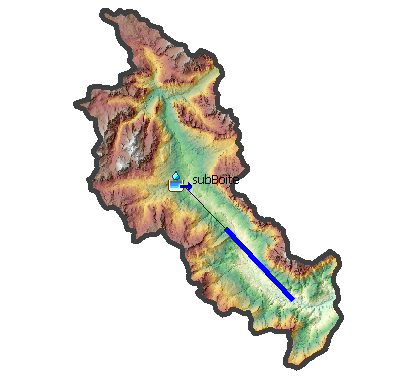
\includegraphics[scale=0.73]{immagini/bac_boite.PNG}
        \caption{Bacino idrografico del Boite.}
    \label{bacino_boite}    
    \end{minipage}
        \hspace{2cm}
    \begin{minipage}[]{7cm}
        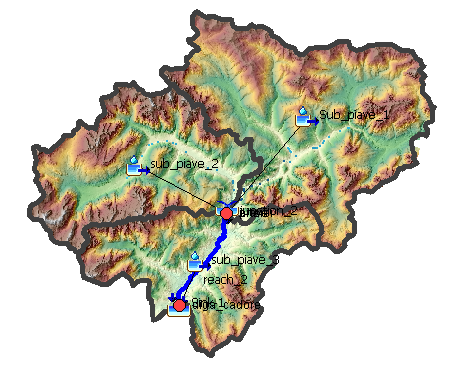
\includegraphics[scale=0.75]{immagini/bac_piave.PNG}
        \caption{Bacino idrografico del Piave.}
    \label{bacino_piave}
    \end{minipage} 
        \end{figure}

Al fine di svolgere in modo più corretto la procedura di analisi spaziale (come verrà descritta successivamente), si è scelto di suddividere il territorio del bacino del Piave in ulteriori tre sottobacini.\\
Il bacino del fiume Boite ha un'estensione di 383 $km^2$, mentre il bacino del Piave ha un'estensione totale di 813 $km^2$.\\
Come verrà ricordato anche successivamente, ai fini della modellazione idraulica è doveroso far presente che all'interno del bacino del Piave sono presenti una serie di invasi artificiali, in grado di modificare l'andamento del deflusso alla sezione di chiusura.